% \iffalse
\let\negmedspace\undefined
\let\negthickspace\undefined
\documentclass[journal,12pt,twocolumn]{IEEEtran}
\usepackage{cite}
\usepackage{amsmath,amssymb,amsfonts,amsthm}
\usepackage{algorithmic}
\usepackage{graphicx}
\usepackage{textcomp}
\usepackage{xcolor}
\usepackage{txfonts}
\usepackage{listings}
\usepackage{enumitem}
\usepackage{mathtools}
\usepackage{gensymb}
\usepackage{comment}
\usepackage[breaklinks=true]{hyperref}
\usepackage{tkz-euclide} 
\usepackage{listings}
\usepackage{gvv}                                        
\def\inputGnumericTable{}                                 
\usepackage[latin1]{inputenc}                                
\usepackage{color}                                            
\usepackage{array}                                            
\usepackage{longtable}                                       
\usepackage{calc}                                             
\usepackage{multirow}                                         
\usepackage{hhline}                                           
\usepackage{ifthen}                                           
\usepackage{lscape}
\usepackage{caption}
\newtheorem{theorem}{Theorem}[section]
\newtheorem{problem}{Problem}
\newtheorem{proposition}{Proposition}[section]
\newtheorem{lemma}{Lemma}[section]
\newtheorem{corollary}[theorem]{Corollary}
\newtheorem{example}{Example}[section]
\newtheorem{definition}[problem]{Definition}
\newcommand{\BEQA}{\begin{eqnarray}}
\newcommand{\EEQA}{\end{eqnarray}}
\newcommand{\define}{\stackrel{\triangle}{=}}
\theoremstyle{remark}
\newtheorem{rem}{Remark}
\begin{document}
\parindent 0px
\bibliographystyle{IEEEtran}
\vspace{3cm}

\title{NCERT 10.5.2 17Q}
\author{EE23BTECH11012 - Chavan Dinesh$^{*}$% <-this % stops a space
}
\maketitle
\newpage
\bigskip

\renewcommand{\thefigure}{\arabic{figure}}
\renewcommand{\thetable}{\arabic{table}}
\large\textbf{\textsl{Question:}}
Find the $20^{th}$ term from the last term of the AP: $3,8,13.....253$.

\solution

As the $20^{th}$ term is considered from last, 

\begin{table}[htbp]
    \centering
    \begin{tabular}{|c|c|c|}
        \hline
        \textbf{Parameter} & \textbf{Description}&\textbf{Value}\\
        \hline
        $x(0)$ & first term  & $253$ \\
         \hline
        $d$ & common difference & $3 - 8 = -5$\\
        \hline
        $x(n)$ & $(n+1)^{th}$ term &($x(0) + nd)u(n)$ \\
        \hline
        $u(n)$  & unit step function  &\\
        \hline
        $x(n)$ & $20^{th}$ term&$158$\\
        \hline
        % $x(N-n)$&$(n+1)^{th}$ term from last &$x(0) + (N - n)d$\\
        % \hline
    \end{tabular}

    \caption{Input table}
    \label{tab:parameter_table.10.5.2.17}
\end{table}
% From \tabref{tab:parameter_table.10.5.2.17}:
% \begin{align}
%     x(n)&=x(0) + nd\\
%      x(19) &= 253 + (-5)19 \\
%         &= 158 
% \end{align}
% From \tabref{tab:parameter_table.10.5.2.17}:
% \begin{align}
% x(N-n)&=x(0) + (N-n)d\\
% x(N-19) &= 3 + (50 - 19)(5)\\
% &= 3 + 155\\
% &= 158
% \end{align}

From equation \eqref{eq:ztrans} and \eqref{eq:11.9.5.26.2}:
\(Z\)-Transform of \(x(n)\):
\begin{align}
 X(z) =\frac{253}{1-z^{-1}}+ \frac{-5z^{-1}}{\brak{1-z^{-1}}^2};\cbrak{z\in\mathbb{C} : |z|>1}
\end{align}

\begin{figure}[ht]
    \centering
    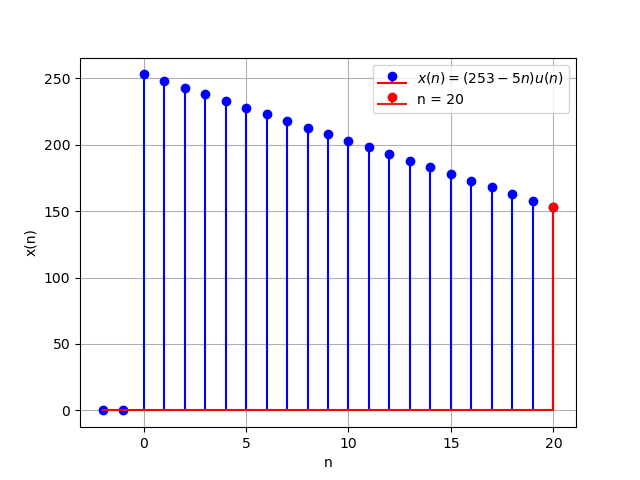
\includegraphics[width = \columnwidth]{figs/x(n)_vs_n.png}
    \caption{}
    \label{fig:graph1}
\end{figure}

\bibliographystyle{IEEEtran}
\end{document}
